%%
%% This is file `tikzposter-template.tex',
%% generated with the docstrip utility.
%%
%% The original source files were:
%%
%% tikzposter.dtx  (with options: `tikzposter-template.tex')
%%
%% This is a generated file.
%%
%% Copyright (C) 2014 by Pascal Richter, Elena Botoeva, Richard Barnard, and Dirk Surmann
%%
%% This file may be distributed and/or modified under the
%% conditions of the LaTeX Project Public License, either
%% version 2.0 of this license or (at your option) any later
%% version. The latest version of this license is in:
%%
%% http://www.latex-project.org/lppl.txt
%%
%% and version 2.0 or later is part of all distributions of
%% LaTeX version 2013/12/01 or later.
%%


\documentclass{tikzposter} %Options for format can be included here

\usepackage{todonotes}

\usepackage[tikz]{bclogo}
\usepackage{lipsum}
\usepackage{amsmath}
\usepackage{fontawesome}
\usepackage{booktabs}
\usepackage{longtable}
\usepackage[absolute]{textpos}
\usepackage[it]{subfigure}
\usepackage{graphicx}
\usepackage{cmbright}
%\usepackage[default]{cantarell}
%\usepackage{avant}
%\usepackage[math]{iwona}
\usepackage[math]{kurier}
\usepackage[T1]{fontenc}
\usepackage{tikz}
%% add your packages here
\usepackage{hyperref}
% for random text
\usepackage{lipsum}
\usepackage[english]{babel}
\usepackage[pangram]{blindtext}

\usepackage{forest}
\usetikzlibrary{arrows.meta, shapes.geometric, calc, shadows}

%% aiming high
%\usepackage{smartdiagram}
%\usetikzlibrary{shapes.symbols}
%
%\tikzset{description title/.append style={
%    signal,
%    signal to=north,
%    signal from=south,
%    yshift=0.5cm,
%  }
%}



\colorlet{mygreen}{green!75!black}
\colorlet{col1in}{red!30}
\colorlet{col1out}{red!40}
\colorlet{col2in}{mygreen!40}
\colorlet{col2out}{mygreen!50}
\colorlet{col3in}{blue!30}
\colorlet{col3out}{blue!40}
\colorlet{col4in}{mygreen!20}
\colorlet{col4out}{mygreen!30}
\colorlet{col5in}{blue!10}
\colorlet{col5out}{blue!20}
\colorlet{col6in}{blue!20}
\colorlet{col6out}{blue!30}
\colorlet{col7out}{orange}
\colorlet{col7in}{orange!50}
\colorlet{col8out}{orange!40}
\colorlet{col8in}{orange!20}
\colorlet{linecol}{blue!60}

\colorlet{backgroundcolor}{blue!10}




 % Title, Author, Institute
\title{Team for Universal Learning and Intelligent Processing}
\author{Gang Li}
\institute{$^1$ School of Information Technology \\
	            Deakin University, Australia
}
%\titlegraphic{logos/tulip-logo.eps}

%Choose Layout
\usetheme{Wave}

%\definebackgroundstyle{samplebackgroundstyle}{
%\draw[inner sep=0pt, line width=0pt, color=red, fill=backgroundcolor!30!black]
%(bottomleft) rectangle (topright);
%}
%
%\colorlet{backgroundcolor}{blue!10}

\begin{document}


\colorlet{blocktitlebgcolor}{blue!23}

 % Title block with title, author, logo, etc.
\maketitle

\begin{columns}
 % FIRST column
\column{0.5}% Width set relative to text width

%%%%%%%%%% -------------------------------------------------------------------- %%%%%%%%%%
 %\block{Main Objectives}{
%  	      	\begin{enumerate}
%  	      	\item Formalise research problem by extending \emph{outlying aspects mining}
%  	      	\item Proposed \emph{GOAM} algorithm is to solve research problem
%  	      	\item Utilise pruning strategies to reduce time complexity
%  	      	\end{enumerate}
%%  	      \end{minipage}
%}
%%%%%%%%%% -------------------------------------------------------------------- %%%%%%%%%%


%%%%%%%%%% -------------------------------------------------------------------- %%%%%%%%%%
\block{TULIP Lab}{
\selectcolormodel{rgb}
\pgfkeys{/forest,
  rect/.append style   = { rounded corners = 2pt,
                         inner color = col6in, outer color = col6out},
  ellip/.append style  = { inner color = col5in,
                          outer color = col5out},
  orect/.append style  = { font = \sffamily\bfseries\LARGE,
                         text width = 325pt, text centered,
                         minimum height = 10pt, outer color = col7out,
                         inner color=col7in},
  oellip/.append style = { inner color = col8in, outer color = col8out,
                          font = \sffamily\bfseries\large, text centered}}
\begin{forest}
  for tree={
      font=\sffamily\bfseries,
      line width=1pt,
      draw=linecol,
      ellip,
      align=center,
      child anchor=north,
      parent anchor=south,
      drop shadow,
      l sep+=12.5pt,
      edge path={
        \noexpand\path[color=linecol, rounded corners=5pt,
          >={Stealth[length=11pt]}, line width=1pt, ->, \forestoption{edge}]
          (!u.parent anchor) -- +(0,-5pt) -|
          (.child anchor)\forestoption{edge label};
        },
      where level={3}{tier=tier3}{},
      where level={0}{l sep-=5pt}{},
      where level={1}{}{},
  }
    [TULIP Academy %inner color=col1in, outer color=col1out
    [Visitor]
    [Flipper
    [Trainee
        [[FLIP (00)]
          [\dots]
          [FLIP (05)]
        ]
    ]]
    [TULIP Lab
        [Australia]
        [China]
        [India]]
    [Alumni] %inner color =col7in, outer color = col7out]
    [Web Team] %, inner color=col2in, outer color=col2out]
  ]
\end{forest}
  	
\begin{description}
\item[Official Websites]
  \begin{itemize}
    \item \textcolor{orange}{\faHome:} \url{http://www.tulip.org.au}
    \item \textcolor{orange}{\faGithub:} \url{https://github.com/tulip-lab}
  \end{itemize}

\item[Social Media]
  \begin{itemize}
    \item \textcolor{orange}{\faTwitter:} \href{https://twitter.com/tulipacademy}{tulipacademy}
    \item \textcolor{orange}{\faWeibo:} \href{https://weibo.com/tulipacademy}{tulipacademy}
    \item \textcolor{orange}{\faRedditAlien:} \url{https://www.reddit.com/r/tulipacademy}
  \end{itemize}


\item[Internal Services]
  \begin{itemize}
   \item \textcolor{orange}{\faBitbucket:} \url{https://bitbucket.org}
   \item \textcolor{orange}{\faCalendar:} \url{https://goo.gl/cWCWwC}
   \item \textcolor{orange}{\faCalendarCheckO:} \url{https://goo.gl/aC9VWW} (iCal)
  \end{itemize}

\end{description}
}
%%%%%%%%%% -------------------------------------------------------------------- %%%%%%%%%%


%%%%%%%%%% -------------------------------------------------------------------- %%%%%%%%%%
\block{Research @ TULIP -   Theme 1.Behavior Informatics}{
\begin{itemize}
    \item
    Case Study(1). Tourist Movement Analysis

    \item
    Case Study(2). Periodic Behavior Mining
    
    \item 
    Case Study(3). Face Age Recognition
    
    \item
    Case Study(4). Speech Based Emotion Detection
    
    \item
    Case Study(5). K Complex Detection
    
    \item
    Case Study(6). Trajectory Analysis  
\end{itemize}

%\begin{figure}[htbp]
%    \subfigure[Asian Tourist]
%    {
%        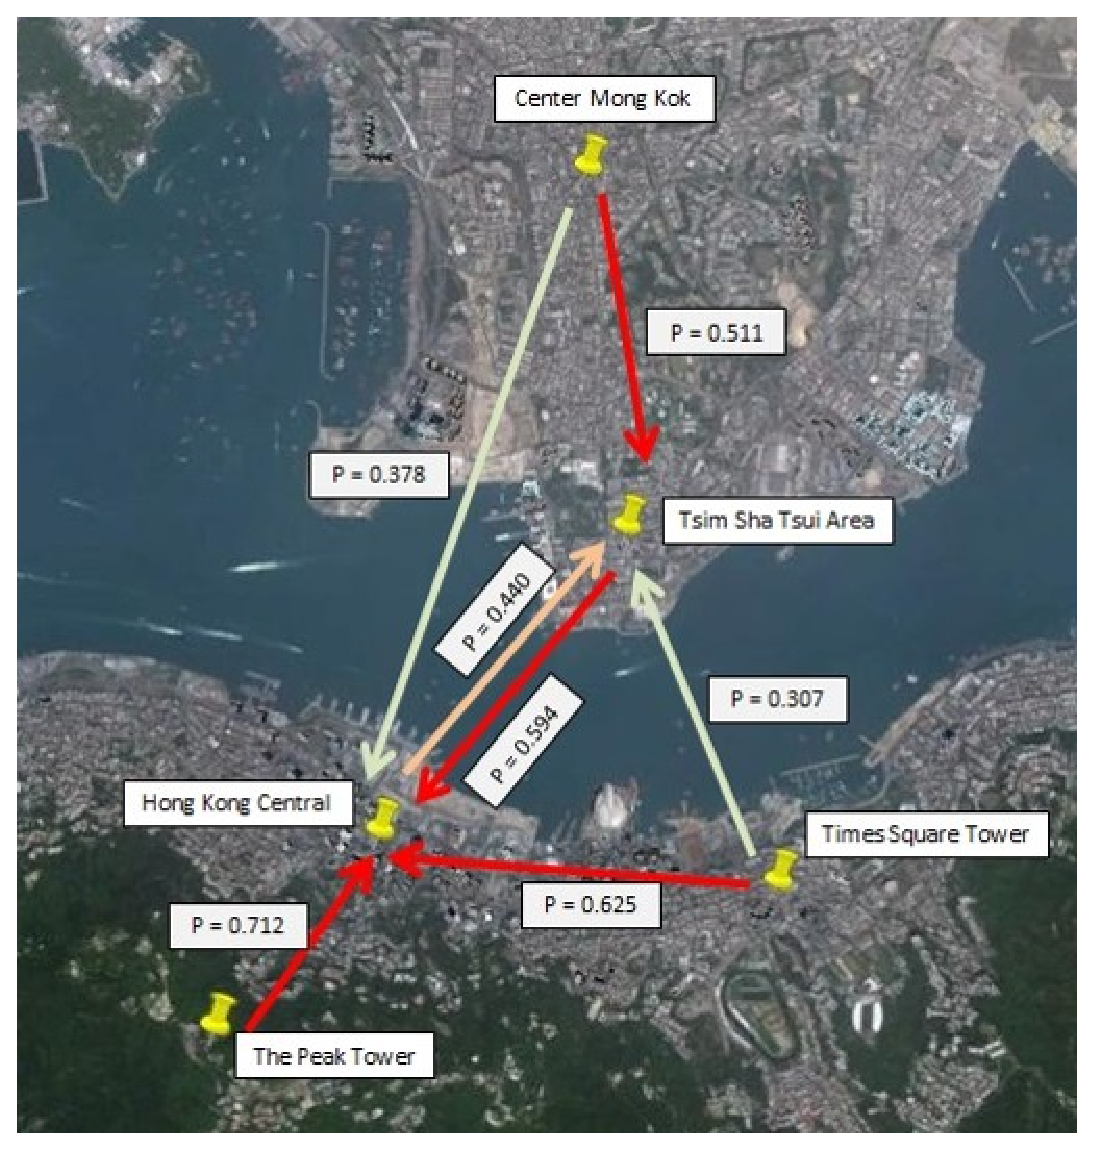
\includegraphics[height=0.4\textwidth,width=0.34\textwidth]{figures//theme1//Theme1_12.eps}
%    }
%    \subfigure[Western Tourist]
%    {
%        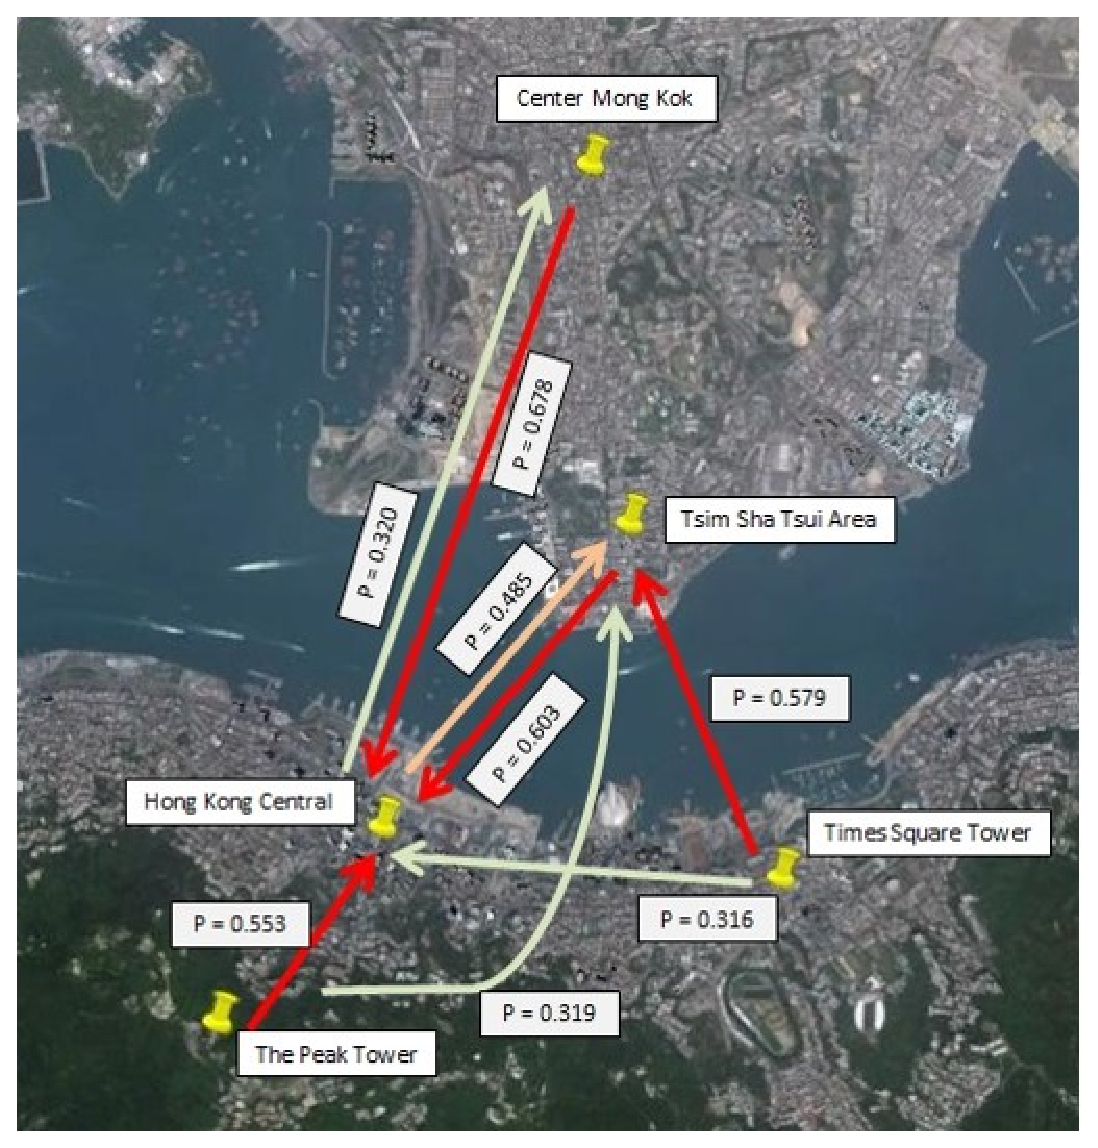
\includegraphics[height=0.4\textwidth,width=0.34\textwidth]{figures//theme1//Theme1_13.eps}
%    }
%\end{figure}


}
%%%%%%%%%% -------------------------------------------------------------------- %%%%%%%%%%


%%%%%%%%%% -------------------------------------------------------------------- %%%%%%%%%%

%\note{Note with default behavior}

%\note[targetoffsetx=12cm, targetoffsety=-1cm, angle=20, rotate=25]
%{Note \\ offset and rotated}

 % First column - second block


%%%%%%%%%% -------------------------------------------------------------------- %%%%%%%%%%
\block{Research @ TULIP -   Theme 2.Data Privacy}{
\begin{itemize}
  \item
  Case Study(1). Is O.S.N. a Secure Place to Show off?
  
  \item
  Case Study(2). Privacy Breach
  
\end{itemize}
}
%%%%%%%%%% -------------------------------------------------------------------- %%%%%%%%%%


% SECOND column
\column{0.5}
 %Second column with first block's top edge aligned with with previous column's top.

%%%%%%%%%% -------------------------------------------------------------------- %%%%%%%%%%
\block{Research @ TULIP -   Theme 3. Business Intelligence}{
\begin{itemize}
  \item
  Case Study(1). Market Segmentation Analysis

  \item
  Case Study(2). Negative Association Rule Mining
  
  \item
  Case Study(3). Contrast Mining
  
  \item 
  Case Study(4). PR Based Conditional Random Fields

\end{itemize}



}
%%%%%%%%%% -------------------------------------------------------------------- %%%%%%%%%%
% Second column - first block


%%%%%%%%%% -------------------------------------------------------------------- %%%%%%%%%%
\block[titleleft]{Awards}
{
\begin{description}
  	\item[Synthetic Dataset] contains $10$ groups and $8$ features.
    Each group consists of $10$ members,
    and each member has $8$ features.
\end{description}
\vspace{.5cm}
\begin{tabular}{ c | c | c | c }
    \toprule
    Method     &  Truth Outlying Aspects    & Identified Aspects & Accuracy      \\
    \midrule
    GOAM       &  $\{F_1\}$, $\{F_2F_4\}$   &  $\{F_1\}$, $\{F_2F_4\}$    & 100\%    \\

     Arithmetic Mean based OAM &  $\{F_1\}$, $\{F_2F_4\}$   &  $\{F_4\}$, $\{F_2\}$    &  0\% \\

     Median based OAM &  $\{F_1\}$, $\{F_2F_4\}$   &  $\{F_2\}$, $\{F_4\}$    &           0\% \\
     \bottomrule
\end{tabular}
\vspace{.2cm}
\begin{description}
    \item
    It can be observed that the GOAM method can identify the trivial outlying features
    and non-trivial outlying subspaces correctly and is obvious from the table
    that the accuracy of GOAM is the best, which is ($100\%$).
\end{description}

\begin{description}
\item[NBA Dataset] was collected from Yahoo Sports
website (\url{http://sports.yahoo.com.cn/nba}).
The data include all teams from the six divisions,
and each player in the team has $12$ features.
\end{description}
\vspace{.5cm}
\begin{tabular}{ c | c | c }
    \toprule
    Teams                   & Trivial Outlying Aspects  & NonTrivial Outlying Aspects    \\
    \toprule
    Cleveland Cavaliers     & \{3FA\}                   & \{FGA, FT\%\}, \{FGA, FG\%\} \\
    Orlando Magic           & \{Stl\}                   & None                         \\
    Milwaukee Bucks         & \{To\}, \{FTA\}           & \{FGA, FTA\}, \{3FA, FTA\}     \\
%    Golden State Warriors   & \{FG\%\}                  & \{FT\%, Blk\}, \{FGA, 3PT\%, FTA\}\\
%    Utah Jazz               & \{Blk\}                   & \{3FA, 3PT\%\}                    \\
    New Orleans Pelicans    & \{FT\%\}, \{FTA\}         & \{FTA, Stl\}, \{FTA, To\}          \\
    \bottomrule
\end{tabular}

\begin{minipage}{0.5\linewidth}
    \centering
    \begin{tikzfigure}
    \missingfigure[figcolor=white]{Testing figcolor}

    {\small{New Orleans Pelicans on FT\%}}
    \end{tikzfigure}%
\end{minipage}
\hfill
\begin{minipage}{0.5\linewidth}
    \centering
    \begin{tikzfigure}
    \missingfigure[figcolor=white]{Testing figcolor}

    {\small{New Orleans Pelicans on FTA}}
    \end{tikzfigure}%
\end{minipage}
\vspace{.2cm}
\begin{description}
\item
\texttt{New Orleans Pelicans} has more players with
lower \{free throw percentage\}, \{free throws attempted\}.
\end{description}
}
%%%%%%%%%% -------------------------------------------------------------------- %%%%%%%%%%


% Second column - second block
%%%%%%%%%% -------------------------------------------------------------------- %%%%%%%%%%
\block[titlewidthscale=1, bodywidthscale=1]
{Training @ TULIP}
{
%\begin{center}
%\selectcolormodel{rgb}
%\smartdiagramset{description title width=2cm,
%set color list={blue!40,blue!30,orange!40},
%description title text width=1.75cm,
%descriptive items y sep=3.5cm,
%description text width=12cm,
%module minimum height=.4cm}
%
%\smartdiagram[descriptive diagram]{
%{\textbf{$\infty$}, \begin{enumerate}
%         \item Proactively meet with supervisor twice per week
%         \item Proactively present and criticize at \textit{TULIP Seminar}
%         \item FLIP (04-05) and FLIP (06-07) completion
%         \item Act as FLIP team leaders and update materials annually
%         \end{enumerate}},
%{\textbf{Trainee}, \begin{enumerate}
%         \item FLIP (02-03) with success on open \href{https://www.kaggle.com}{Kaggle} projects
%         \item Feedback and suggestions on FLIP
%         \item Present at \textit{TULIP Seminar}
%         \end{enumerate}},
%{\textbf{Flipper},\begin{enumerate}
%         \item \LaTeX + \faGithub \faBitbucket + Time management + PPR skill
%		 \item Keep FLIP materials confidential without distribution
%         \item FLIP (00-01) with success on open \href{https://www.kaggle.com}{Kaggle} projects
%         \item Attend \textit{TULIP Seminar} with preparation and questions
%         \end{enumerate}},}
%\end{center}
}
%%%%%%%%%% -------------------------------------------------------------------- %%%%%%%%%%


% Bottomblock
%%%%%%%%%% -------------------------------------------------------------------- %%%%%%%%%%
\colorlet{notebgcolor}{blue!20}
\colorlet{notefrcolor}{blue!20}
\note[targetoffsetx=8cm, targetoffsety=-4cm, angle=30, rotate=15,
radius=2cm, width=.26\textwidth]{
Acknowledgement
\begin{itemize}
    \item
    International Cooperation Project (Y7Z0511101)
    of IIE,
    Chinese Academy of Sciences
 \end{itemize}
}

%\note[targetoffsetx=8cm, targetoffsety=-10cm,rotate=0,angle=180,radius=8cm,width=.46\textwidth,innersep=.1cm]{
%Acknowledgement
%}

%\block[titlewidthscale=0.9, bodywidthscale=0.9]
%{Acknowledgement}{
%}
%%%%%%%%%% -------------------------------------------------------------------- %%%%%%%%%%

\end{columns}


%%%%%%%%%% -------------------------------------------------------------------- %%%%%%%%%%
%[titleleft, titleoffsetx=2em, titleoffsety=1em, bodyoffsetx=2em,%
%roundedcorners=10, linewidth=0mm, titlewidthscale=0.7,%
%bodywidthscale=0.9, titlecenter]

%\colorlet{noteframecolor}{blue!20}
\colorlet{notebgcolor}{blue!20}
\colorlet{notefrcolor}{blue!20}
\note[targetoffsetx=-13cm, targetoffsety=-12cm,rotate=0,angle=180,radius=8cm,width=.96\textwidth,innersep=.4cm]
{
\begin{minipage}{0.3\linewidth}
\centering
\includegraphics[width=24cm]{logos/tulip-wordmark.eps}
\end{minipage}
\begin{minipage}{0.7\linewidth}
{ \centering
 \large{\textcolor{blue!80}{Welcome to \emph{Team for Universal Learning and
 Intelligent Processing}!}}
}
\end{minipage}
}
%%%%%%%%%% -------------------------------------------------------------------- %%%%%%%%%%


\end{document}

\endinput
%%
%% End of file `tikzposter-template.tex'.
